\documentclass[]{scrartcl}
\title{Vorlesung Analysis II}
\usepackage{amsmath,amssymb,amsfonts}
\usepackage{stmaryrd}
\usepackage{mathtools}
\usepackage{latexsym}
\usepackage{graphicx}
\usepackage{tikz}
\usepackage{xcolor}
\usepackage[most]{tcolorbox}
\usepackage{soul}
\usepackage{ upgreek }
\usepackage{hyperref}
\usepackage{tipa}
\usepackage[dvipsnames]{xcolor}
\hypersetup{
	colorlinks=true,
	linkcolor=blue,
	filecolor=magenta,      
	urlcolor=cyan,
	pdftitle={Overleaf Example},
	pdfpagemode=FullScreen,
}
\newcommand{\redcircle}[1]{%
	\tikz[baseline=(char.base)]{
		\node[shape=circle, draw=red, text=red, thick, inner sep=1pt] (char) 
		{\textbf{#1}};
	}%
}
\newcommand{\bluecircle}[1]{%
	\tikz[baseline=(char.base)]{
		\node[shape=circle, draw=blue, text=blue, thick, inner sep=1pt] (char) 
		{\textbf{#1}};
	}%
}
\newcommand{\blackcircle}[1]{%
	\tikz[baseline=(char.base)]{
		\node[shape=circle, draw=black, text=black, thick, inner sep=1pt] 
		(char) 
		{\textbf{#1}};
	}%
}
\newcommand{\orangecircle}[1]{%
	\tikz[baseline=(char.base)]{
		\node[shape=circle, draw=orange, text=orange, thick, inner sep=1pt] 
		(char) 
		{\textbf{#1}};
	}%
}
\newcommand{\redul}[1]{\setulcolor{red}{\ul{#1}}}
\newcommand{\blueul}[1]{\setulcolor{blue}{\ul{#1}}}
\newcommand{\yelul}[1]{\setulcolor{yellow}{\ul{#1}}}
\newcommand{\greenul}[1]{\setulcolor{green}{\ul{#1}}}
\newcommand{\oraul}[1]{\setulcolor{orange}{\ul{#1}}}
\setul{1pt}{3pt} % Linienhöhe und Abstand zum Text (optional anpassbar)

\setlength{\topmargin}{-.5in} \setlength{\textheight}{9.25in}
\setlength{\oddsidemargin}{0in} \setlength{\textwidth}{6.8in}
\setlength{\parindent}{0pt}

\begin{document}
	\maketitle
	\textbf{\underline{Teil 3: Gewöhnliche Differentialgleichungen}}\\
	\\
	\textbf{\underline{an17: DGLn mit "getrennten Variablen"}}\\
	\\
	\textbf{\underline{\underline{Stichworte:} DGL mit getrennten Variablen, AWA, Beispiele}}\\
	\\
	\textbf{\underline{Literatur}} \blueul{[Hoffmann], Kapitel 7.2}\\
	\\
	\textbf{17.1. \underline{Einleitung:}} Wir untersuchen DGLn mit "getrennten Variablen" x und y.\\
	\\
	\textbf{17.2. \underline{Motivation:}} wir behandeln DGLn, wo sich alle Terme y und ihren Ableitungenauf die eine Seite, und die Terme mit x auf die andere Seite bringen lassen. Nach einer solchen "Variablentrennung" ist die DGL leicht lösbar Integration.\\
	\\
	\textbf{17.3. \underline{Verinbarung:}} Wir betrachtten DGLn der Form\\
	\begin{figure}[h]

		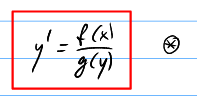
\includegraphics[width=3 cm,height=2cm]{bsp kap 17.3}
	\end{figure}\\ 
	\underline{Annahmen:} $i_1.i_2\subseteq \mathbb{R}$ Intervalle,\\
	$f:i_1\rightarrow\mathbb{R}$ \underline{stetig}, $g:i_2\rightarrow\mathbb{R}$ \underline{stetig} mit \underline{$g(s)\neq0$ für $s\in i_2$}.\\
	\\
	\textbf{17.4. \underline{Aufgabe:}} Zu den Anfangswerten $a\in i_1$ und $b \in i_2$ suchen wir ein $IV i\subseteq \mathbb{R}$ mit $a\in i \subseteq i_1$ und eine auf i def. Lsg. y von \blackcircle{*} mit \redul{y(a)=b}.\\
	\redul{"AWA"=Anfangswertaufgabe}\\
	\\
	\textbf{17.5. \underline{Grobe Idee:}} Umformung zu $y'(t)g(y(t))=f(t)$\\
	und Integration: $\int_{a}^{x}y'(t)g(y(t))dt=\int_{a}^{x}f(t)dt$.\\
	Die Substitution $s:=y(t)$ ergibt auf der l.s. gerade $\int_{y(a)}^{y(x)}g(s)ds$,\\
	was dann nach y(x) aufgelöst wird.\\
	\\
	\textbf{17.6. \underline{Bemerkung:}}\\
	(1.) Durch "Variazion" von a und b werden \underline{alle} Lsgn. erfasst.\\
	(2.) Eine Lsg. von \blackcircle{*} ist automatisch stetig diff'bar.\\
	\\
	\textbf{17.7.} Setze \yelul{F(x)}:=$\int_{a}^{x}f(t)dt (x\in i_1)$, \yelul{G(y)}:=$\int_{b}^{y}g(s)ds (y\in i_2)$-\\
	Da g in $i_2$ keine Nst. hat (und daher Konstantes VZ hat, denn g ist stetig), ist \greenul{G streng monoton} (isoton oder antiton).\\
	G ist stetig diff'bar, für \redul{$i_3$}:=$G(i_2)$ ist also G:$I_2\rightarrow i_3$ \greenul{bijektiv}.\\
	Nach \blueul{An12.2./an8.8.} ist $G^{-1}: i_3\rightarrow i_2$ \greenul{stetig diff'bar}, und ebenso \greenul{streng monoton}.\\
	\\
	\textbf{17.8. \underline{Feststellung:}} Für eine auf einem IV (Intervall) i, $a\in i\subseteq i_1$, def. diff'bare Fkt. y mit $y(t)\in i_2 (t\in i)$ ist die AWA äquivalent zu \fcolorbox{red}{white}{$G(y(x)))F(x), x\in i$} $\Leftrightarrow$ \greenul{$y(x)= G^{-1}(F(x))=(G^{-1}\circ F)(x)$}, $x\in i.$\\
	Ist nun $i_0$ das "maximale" IV mit $a\in i_0 ßsubseteq i_1$ und $F(x)\in i_3, x\in i_0,$ \\
	dann gilt: \redul{$y_0:=G^{-1}\circ F_{ri_0}$}\greenul{ist Lsg. der AWA}.\\
	\greenul{Jede andere Lsg. der AWA entsteht durch Einschränkung.}\\
	\\
	\textbf{17.9. \underline{Bsp.:}}\fcolorbox{red}{white}{$y'=-\frac{x}{y}$}, $y\textgreater0, \rightarrow$ nehmen $i_2=\mathbb{R}, f(x)=-x, i_2=]0,\infty[, g(y)=y$\\
	und bel. $a\in i_1, b\in i_2$, erhalten: \greenul{$2F(x)=-x^2+a^2, 2G(y)=y^2-b^2$},\\
	und somit $i_3=G(i_2)=]-\frac{1}{2}b^2,\infty[.$ mit \redul{$r=\sqrt{a^2+b^2}$} ergibt sich $i_0=]-r,r[$.\\
	Die Forderung \greenul{G(y(x))=F(x)} liefert $y(x)^2-b^2=-x^2+a^2\Rightarrow$  \greenul{$y(x)=\sqrt{r^2-x^2}, x\in i_0$}.\\
	\\
	\textbf{17.10. \underline{Bsp.:}}\fcolorbox{red}{white}{$y'=\sqrt{y}$}, $y \geq 0, y(0)=0 \rightarrow$ Nehmen $i_1=\mathbb{R}, i_2=]0,\infty[,$\\
	\greenul{f(x):=1} $(x\in i_1)$, \greenul{$g(s):=s^{\frac{-1}{2}}$} $(s\in i_2)$.\\
	$\bullet$ \underline{Für b=0} sind wegen $0\notin i_2$ obige Überlegung nicht anwendbar.\\
	$\bullet$ \underline{Falls $a\in i_1, b \in i_2$:} Setze \greenul{F(x):=} $\int_{b}^{y}f(t)dt=$\greenul{x-a}, $x\in i_1$,\\
	\greenul{G(y):}=$\int_{b}^{y} s^{-1/2}ds=$ \greenul{$2(\sqrt{y}-\sqrt{b})$}, $y\in i_2$,\\
	$i_3 (:=G(i_2))=]-2\sqrt{b},\infty[, i_0=]a-2\sqrt{b},\infty[,$\\
	\greenul{$y_0(x):=G^{-1}(F(x))=\frac{1}{4}(x-a+2\sqrt{b})^2$}, $x\in i_0$.\\
	Mit \redul{$\alpha:= a-2\sqrt{b}$} liefert dann \greenul{y(x):=}$\begin{cases}
		0, x\leq \alpha\\
		\frac{1}{4}(x-\alpha), x\textgreater \alpha
	\end{cases}$ einer \greenul{Lsg. auf ganz $\mathbb{R}$}.\\
	\\
	\textbf{17.11. \underline{Bem. zu} \blueul{17.10:}} Falls $\alpha\geq 0$, erhält man eine Lsg.\\
	Es ex. also lokal (hier z.B. um die 0 herum) \greenul{unendlich viele Lsgn. der AWA},\\
	diese liegen zwischen der "Kleinsten" Lsg. $y_{min}=0$ und der "größten" Lsg. $y_{max}(x):=\begin{cases}
		0,x\leq0\\
		\frac{1}{4}x^2, x\textgreater 0.
	\end{cases}$\\
	\begin{figure}[h]
		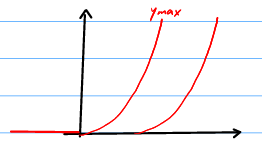
\includegraphics[width=4 cm,height=3cm]{bsp kap 17.11}
	\end{figure}\\
	\\
	\textbf{17.12. \underline{Bsp.:}} \fcolorbox{red}{white}{$y'=y^2$}, $y(0)=b\textgreater0. \rightarrow$ Nehmen $i_1=\mathbb{R}, i_2=]0,\infty[m$\\
	\greenul{f(x)=1} $(x\in i_1)$, \greenul{$g(s)=s^{-2}$}($s\in i_2$), a=0.\\
	Setzen $F(x)=\int_{0}^{x}f(t)dt=x, x\in i_1,\\
	G(y)=\int_{b}^{y}s^{-2}ds=\frac{1}{b}-\frac{1}{b}, y\in i_2$,\\
	$i_3= G(i_2)=]-\infty,\frac{1}{b}[=i_0,$ \greenul{$y_0(x):=G^{-1}(F(x))=G^{-1}(x)=\frac{b}{1-bx}$}, 	$x\in i_0.$\\
	\underline{Beachten:} Die Lsgn. besitzen individuelle maximale existenz IVe, obwohl die DGL mit völlig regulären Funktionen gebildet wird.\\
	\begin{figure}[h]
		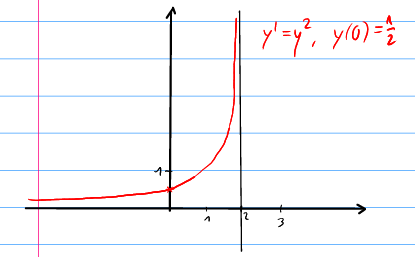
\includegraphics[width=5 cm,height=4cm]{bsp kap 17.12}
	\end{figure}\\
	
	
	
	
	
	
	
	
	
	
	
	
	
	
	
	
	
\end{document}